\renewcommand{\thechapter}{\Alph{chapter}} 
\phantomsection
\addcontentsline{toc}{chapter}{Anhang}
\chapter*{Anhang}
\setcounter{chapter}{1} \setcounter{figure}{0} 
\renewcommand{\chaptermark}[1]{\markboth{\MakeUppercase{#1}}{}}
\renewcommand{\sectionmark}[1]{\markright{\MakeUppercase{#1}}}
\chaptermark{Anhang}

\section*{Abbildungen}
\sectionmark{Abbildungen}
\addcontentsline{toc}{section}{Abbildungen}

\begin{figure}[H]\centering
    \includetikz[0.95]{figures/appendix/fsm}%
    \caption{Vollständige Zustandsmaschine des Caches}
    \label{img:fsm3}
\end{figure} 

\begin{figure}[H]\centering
    \includetikz{figures/chapter7/time4}%
    \caption{Benchmarkergebnisse des Caches für $m=4$}
    \label{img:time4}
\end{figure}

\begin{figure}[H]\centering
    \includetikz{figures/chapter7/time8}%
    \caption{Benchmarkergebnisse des Caches für $m=8$}
    \label{img:time8}
\end{figure}

\begin{figure}[H]\centering
	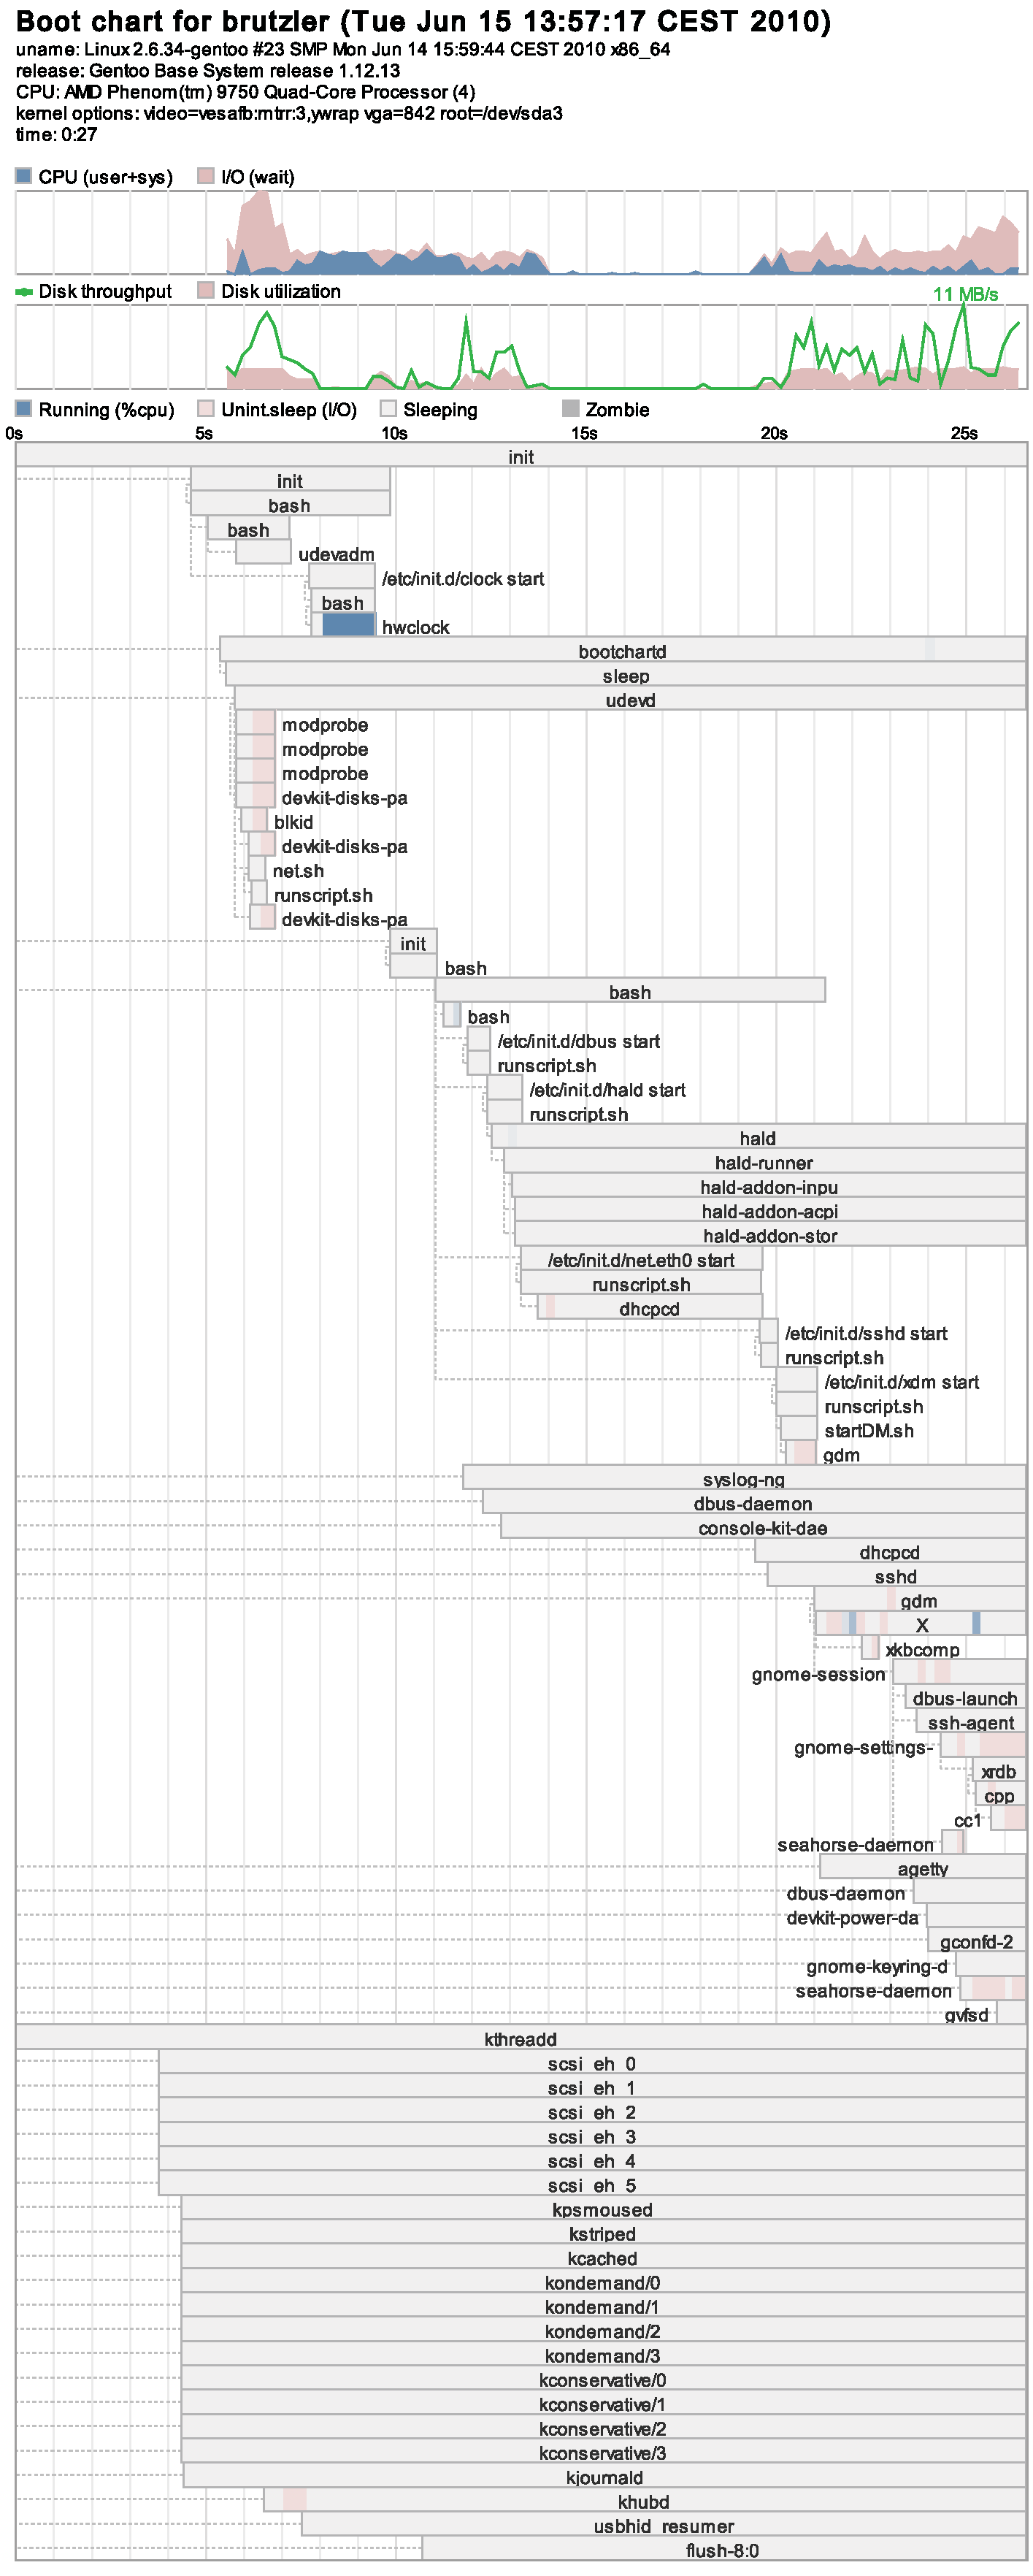
\includegraphics[scale=0.4]{figures/appendix/bootchart-hdd}
    \caption{Ausführliches Log eines HDD-Bootvorgangs}
    \label{img:bootchart-hdd}
\end{figure}

\begin{figure}[H]\centering
	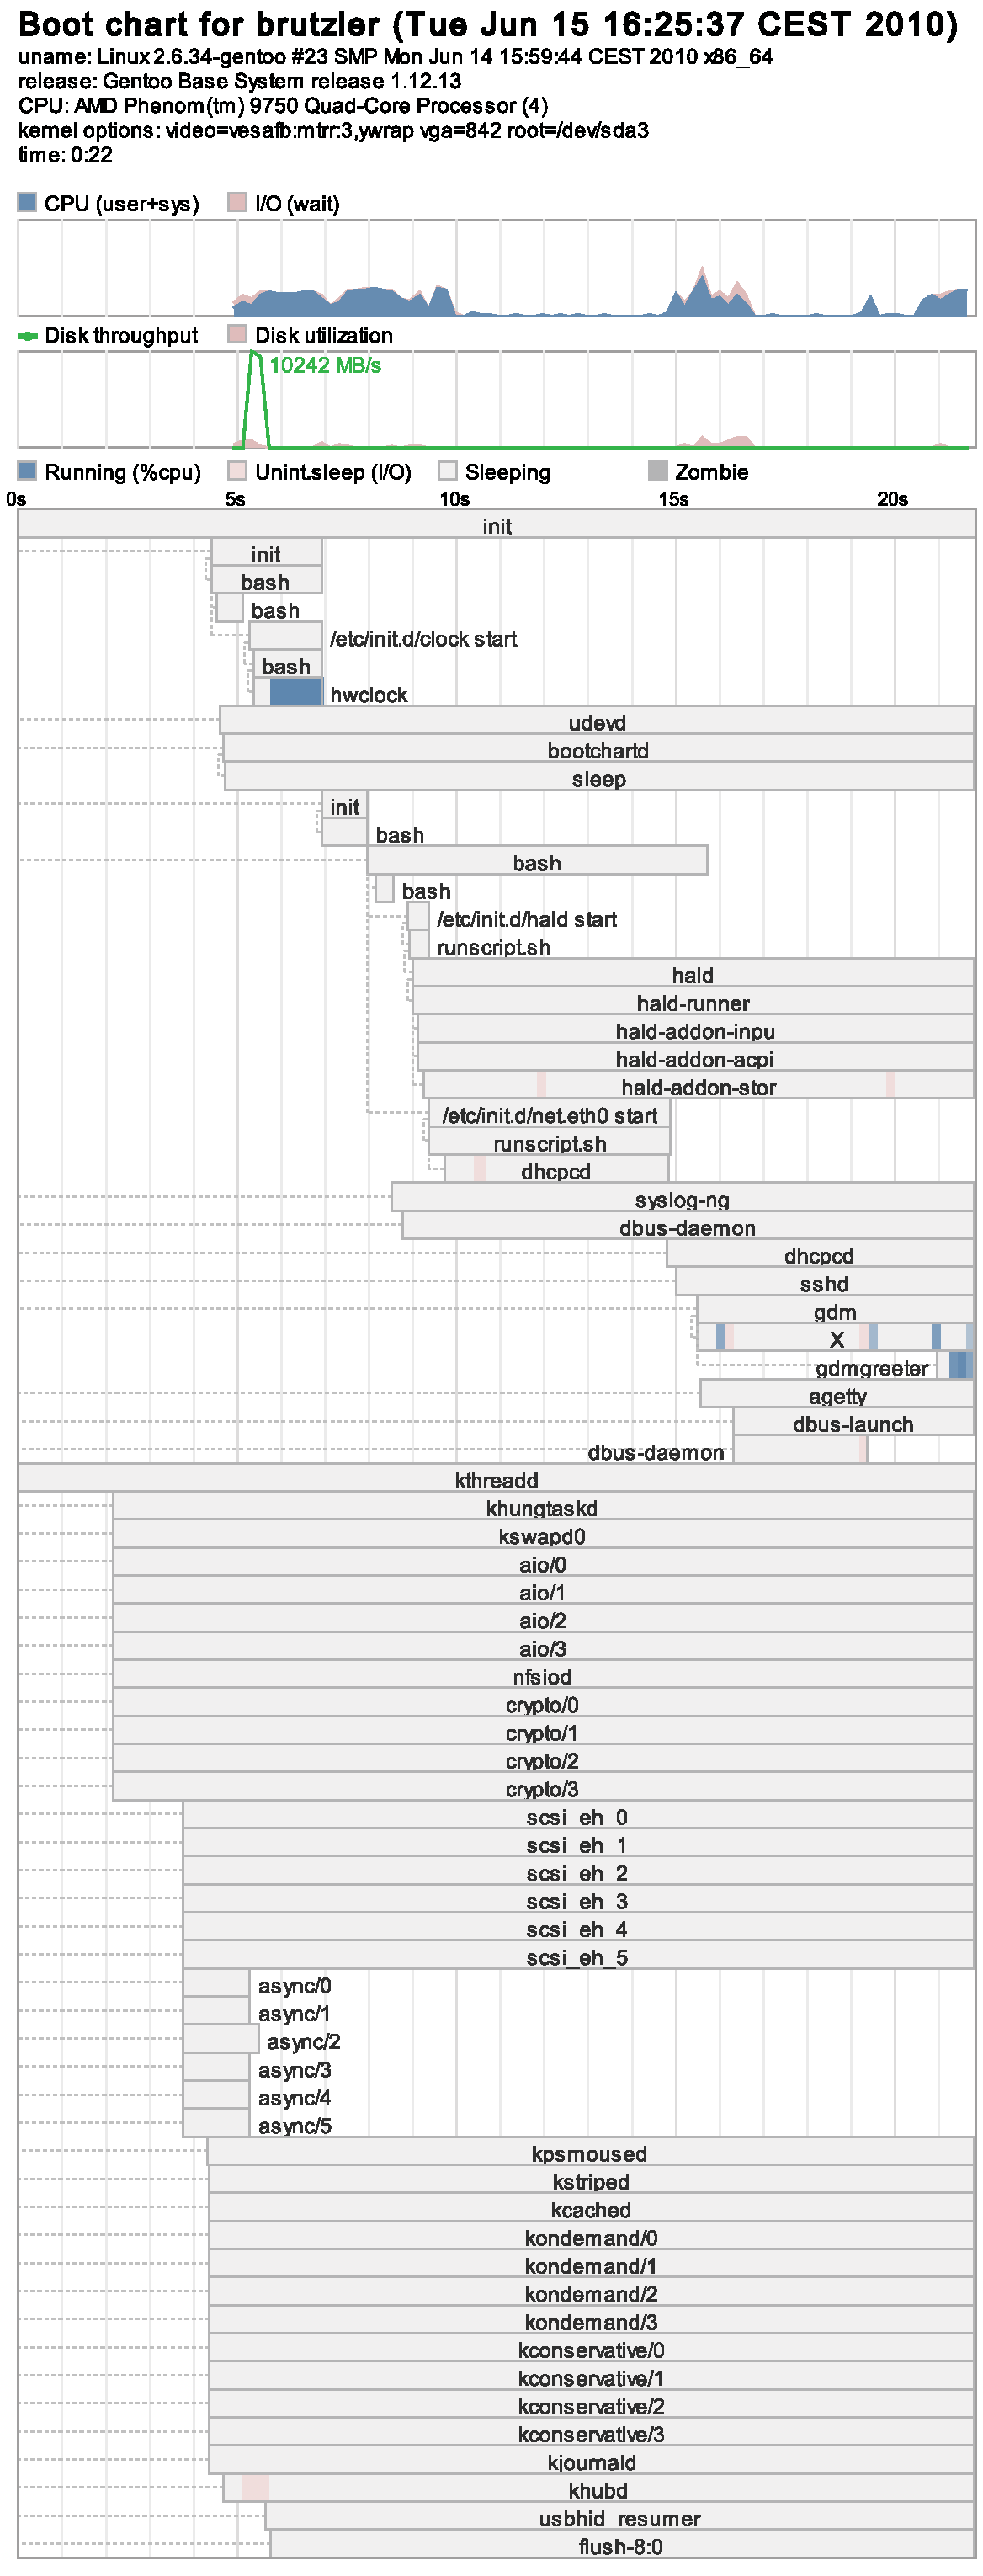
\includegraphics[scale=0.4]{figures/appendix/bootchart-ssd}
    \caption{Ausführliches Log eines SSD-Bootvorgangs mit OCZ SSD}
    \label{img:bootchart-ssd}
\end{figure}

\begin{figure}[H]\centering
	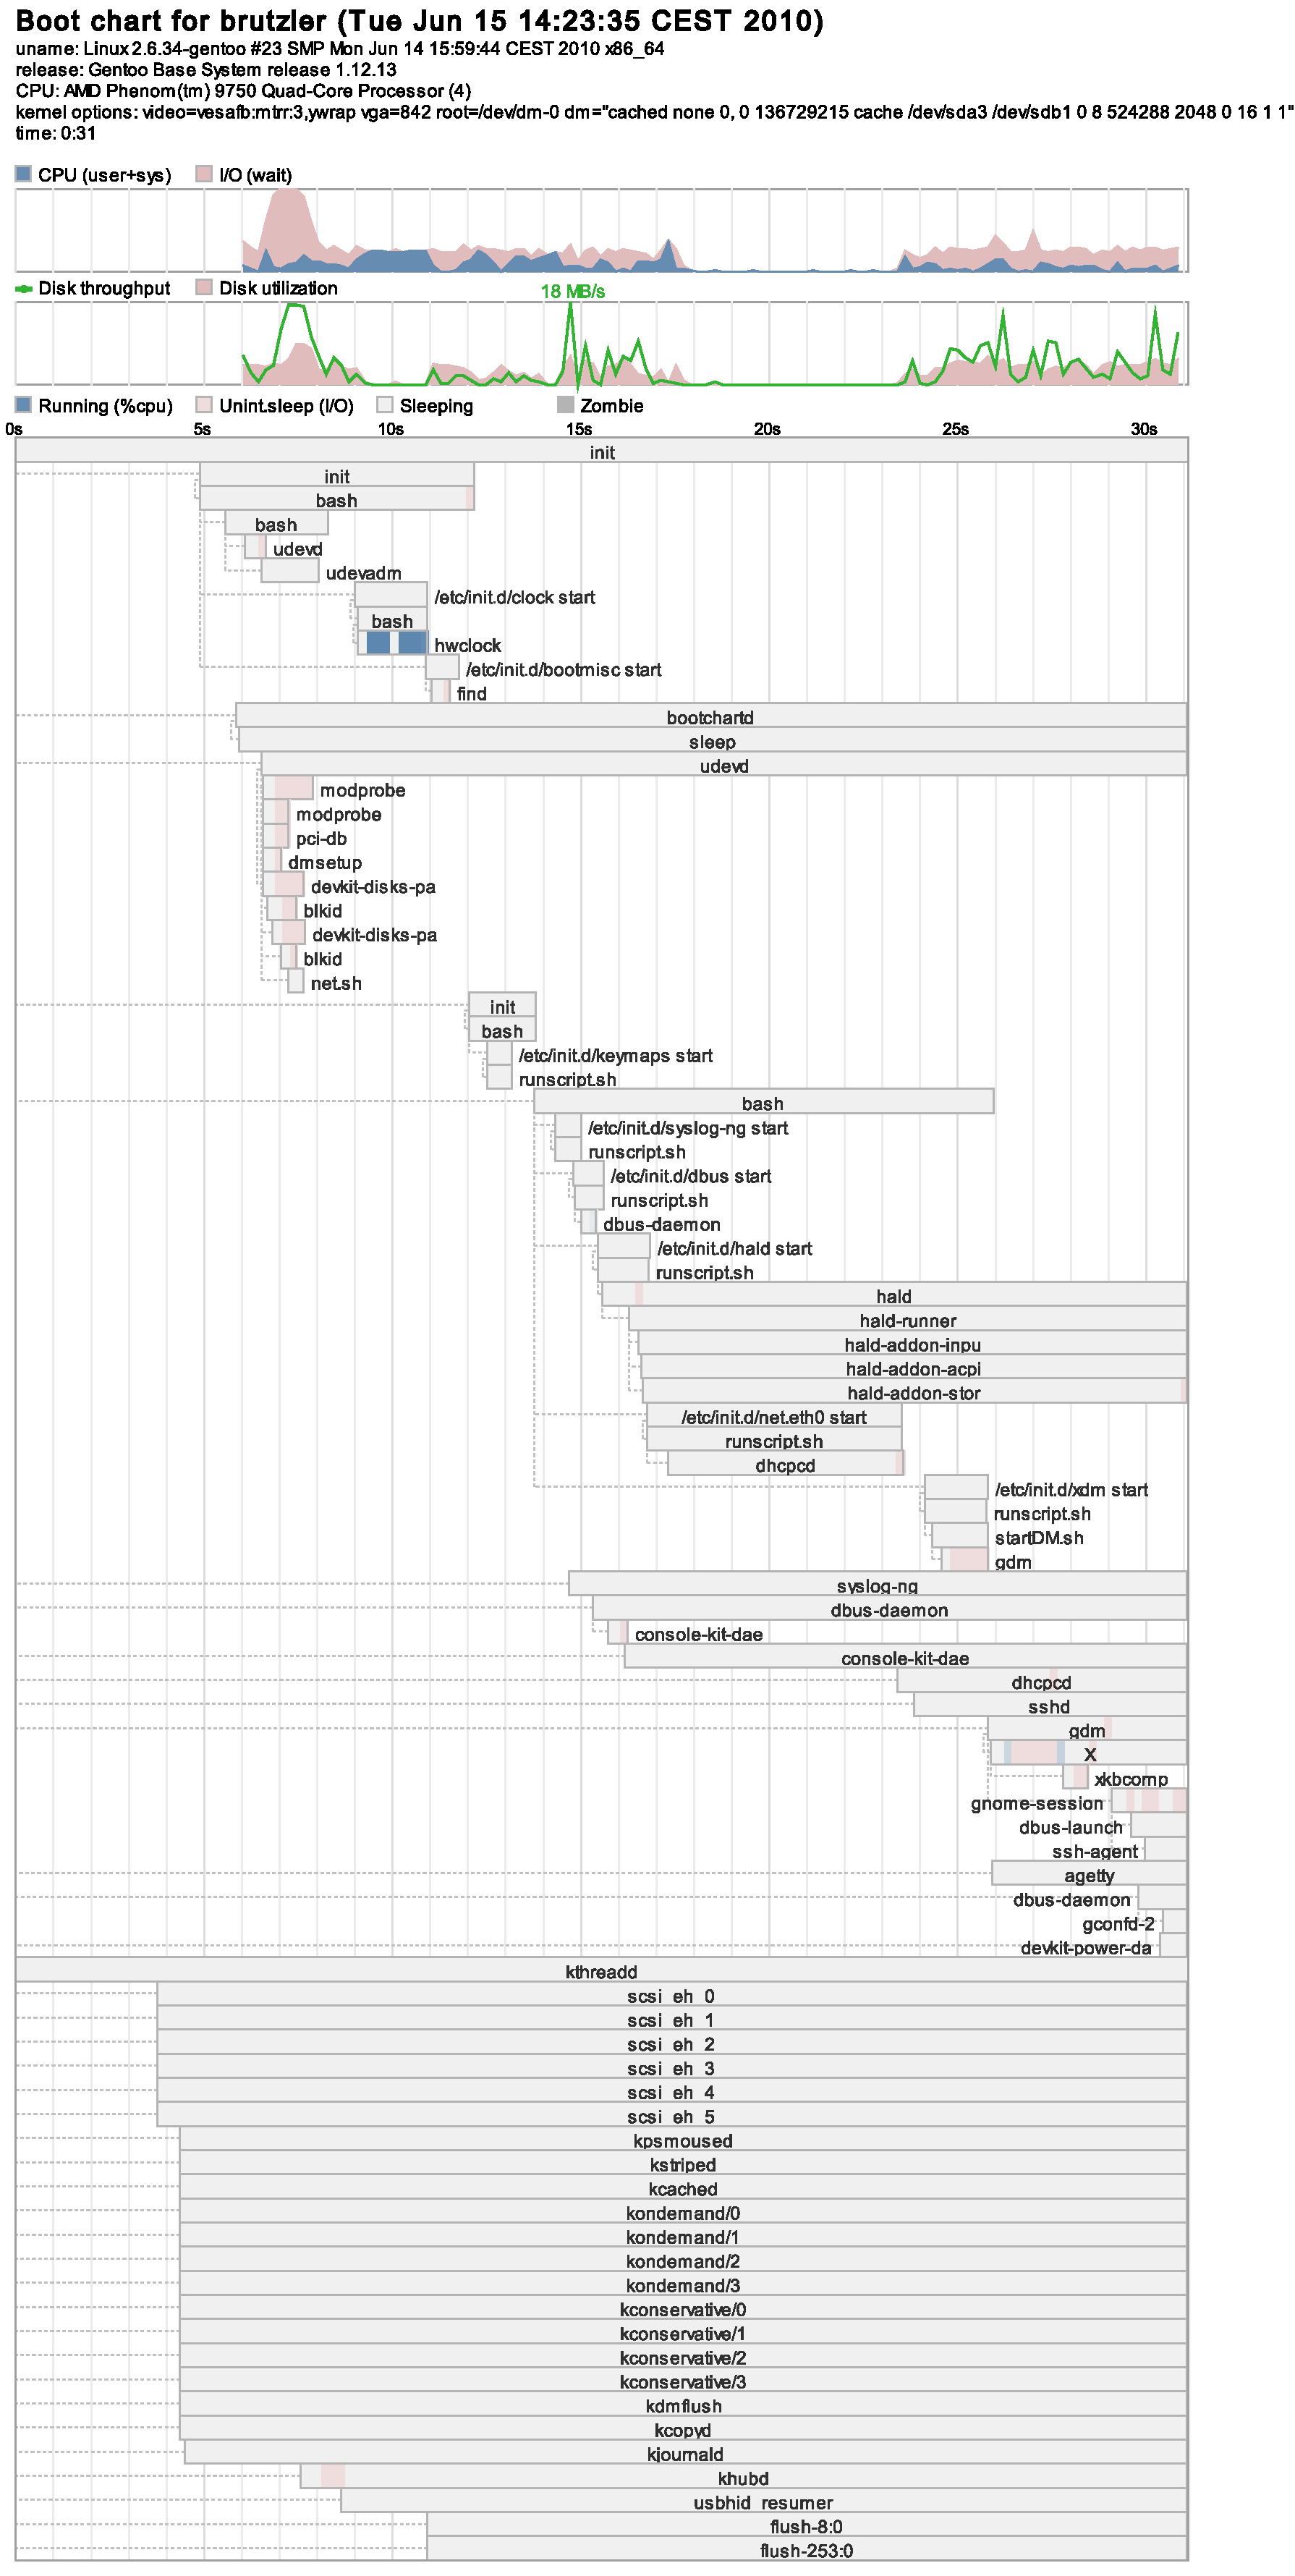
\includegraphics[scale=0.4]{figures/appendix/bootchart-cache1}
    \caption{Ausführliches Log des ersten Cache-Bootvorgangs mit OCZ SSD}
    \label{img:bootchart-cache1}
\end{figure}

\begin{figure}[H]\centering
	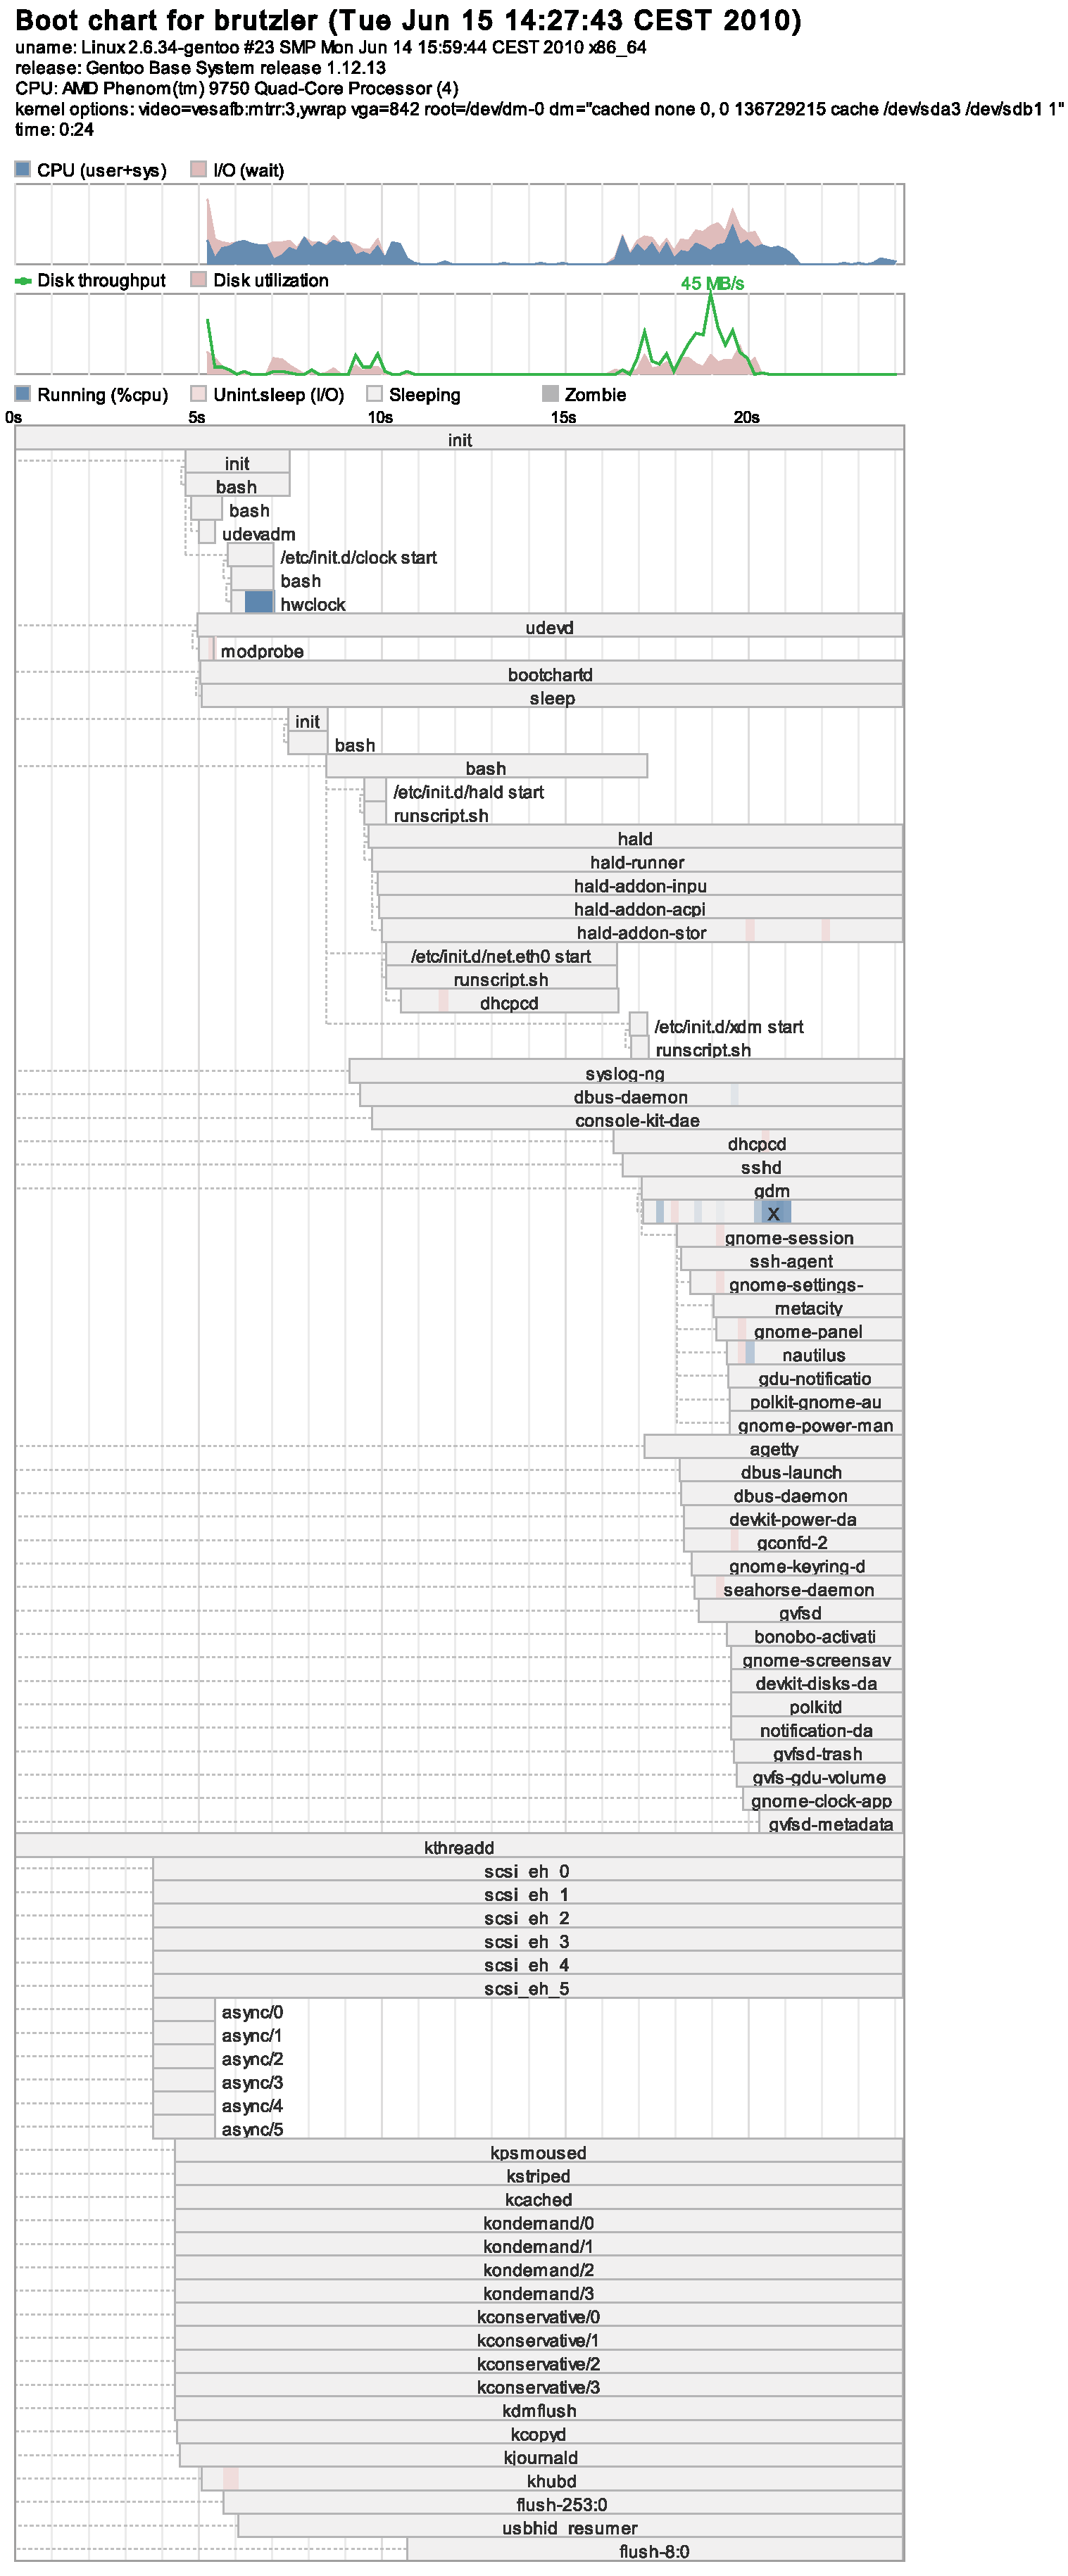
\includegraphics[scale=0.4]{figures/appendix/bootchart-cache2}
    \caption{Ausführliches Log des zweiten Cache-Bootvorgangs mit OCZ SSD}
    \label{img:bootchart-cache2}
\end{figure}

\begin{figure}[H]\centering
	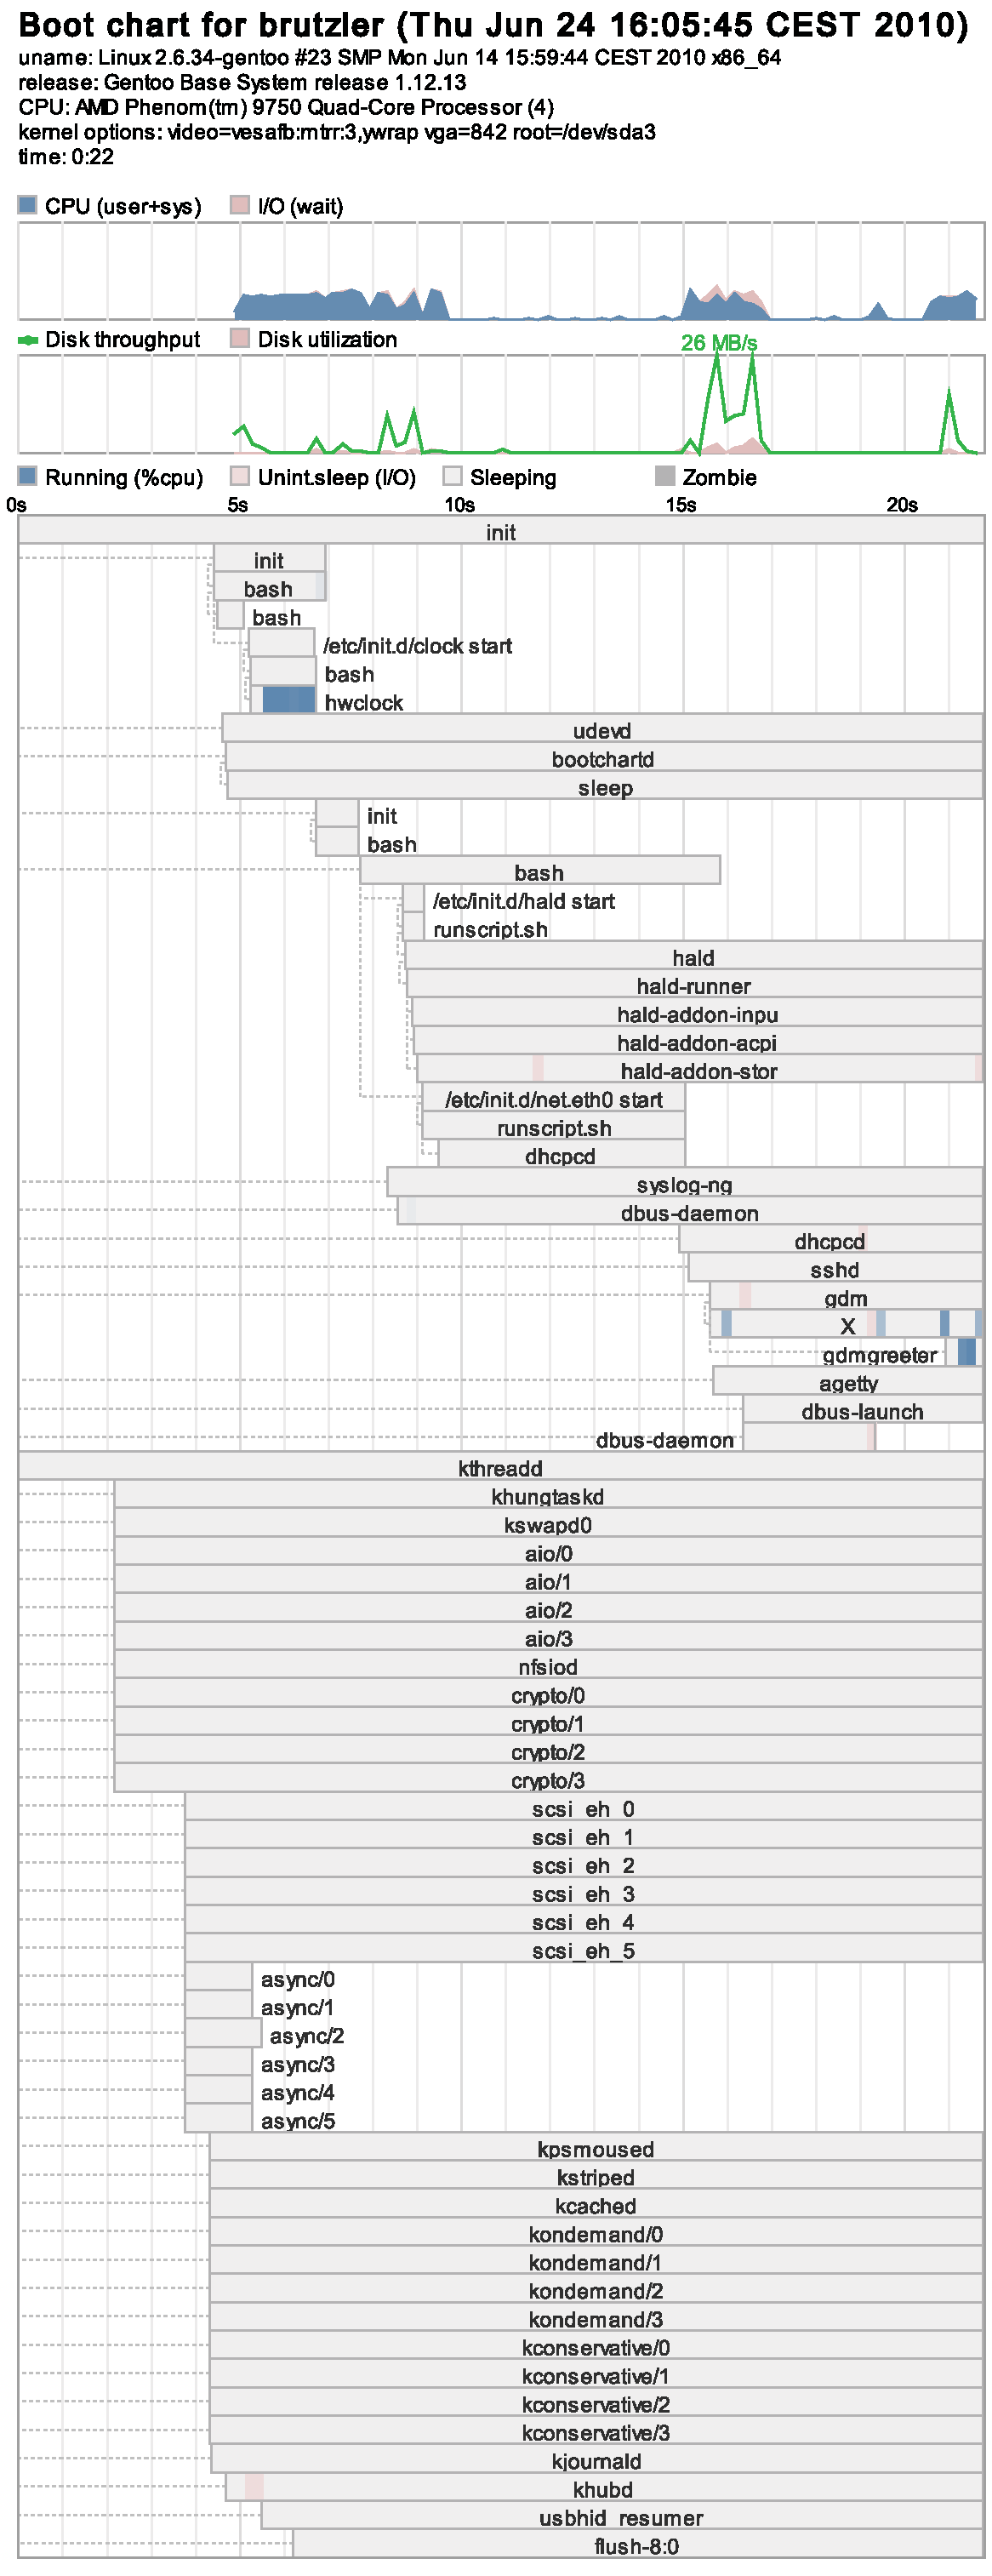
\includegraphics[scale=0.4]{figures/appendix/bootchart-ssd_intel}
    \caption{Ausführliches Log eines SSD-Bootvorgangs mit Intel SSD}
    \label{img:bootchart-ssd:intel}
\end{figure}

\begin{figure}[H]\centering
	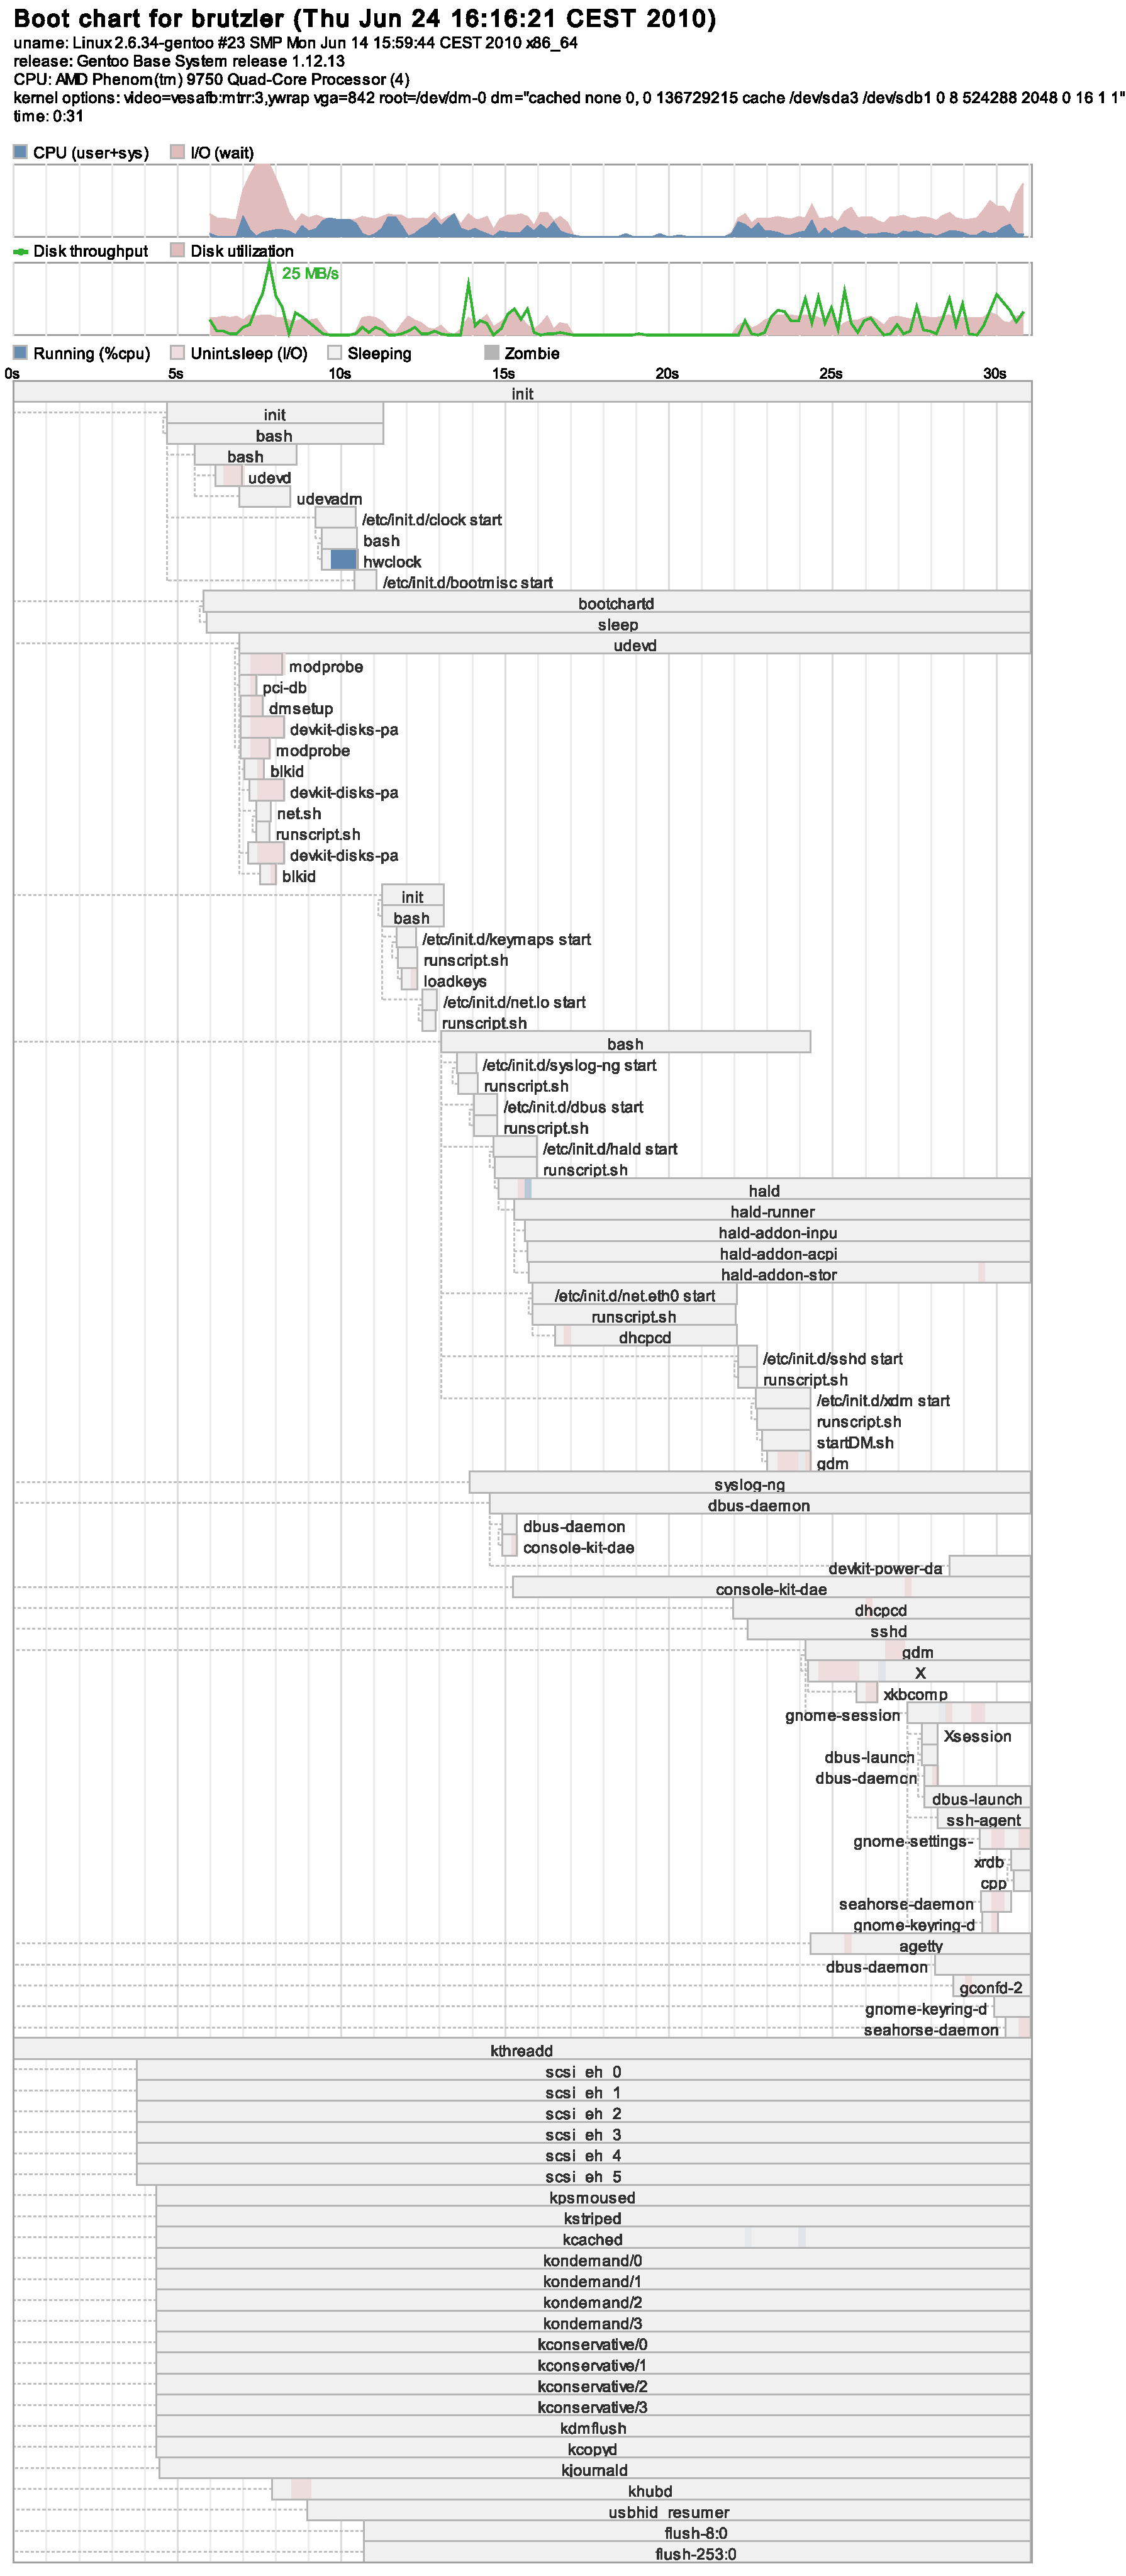
\includegraphics[scale=0.35]{figures/appendix/bootchart-cache1_intel}
    \caption{Ausführliches Log des ersten Cache-Bootvorgangs mit Intel SSD}
    \label{img:bootchart-cache1:intel}
\end{figure}

\begin{figure}[H]\centering
	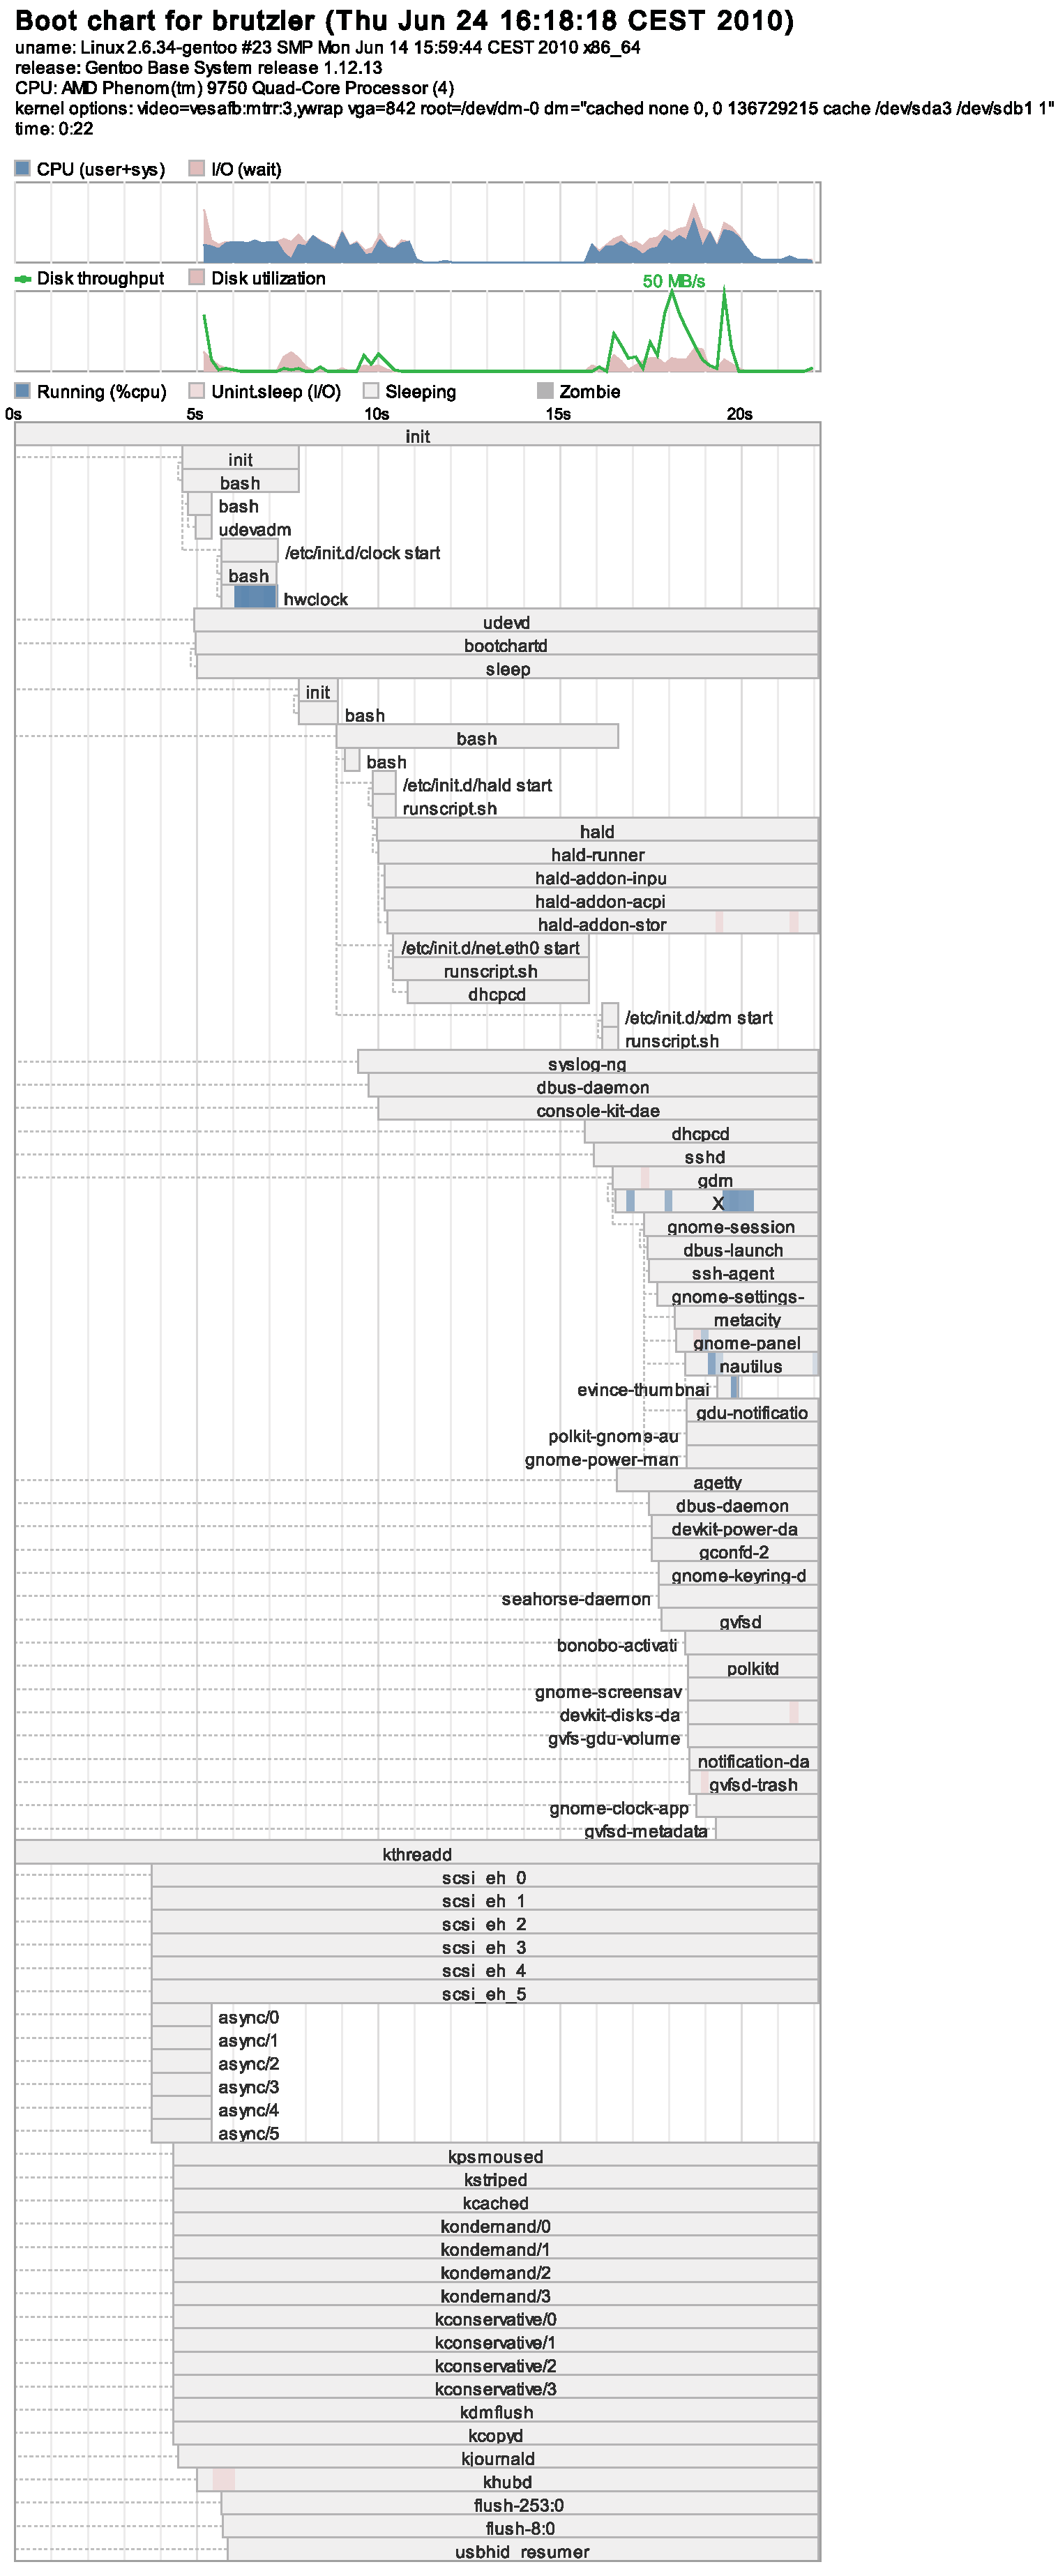
\includegraphics[scale=0.4]{figures/appendix/bootchart-cache2_intel}
    \caption{Ausführliches Log des zweiten Cache-Bootvorgangs mit Intel SSD}
    \label{img:bootchart-cache2:intel}
\end{figure}

\section*{Listings}
\sectionmark{Listings}
\addcontentsline{toc}{section}{Listings}

\subsection*{Linux Kernel}

\lstinputlisting[frame=trbl,caption=Kernelinterne Respräsentation eines \ac{BIO} (Quelle: \cite{src:linux}), label=listing:bio]{listings/struct_bio.source}

\newpage

\subsection*{dm-cache Modul}

\begin{minipage}{\textwidth}
\lstinputlisting[frame=trbl,caption=Datenstruktur für Cachemetainformationen (Quelle: \cite{src:dm-cache}), label=listing:cache1:meta]{listings/struct_cache_c1.source}

\lstinputlisting[frame=trbl,caption=Datenstruktur für Cacheblock-Metainformationen (Quelle: \cite{src:dm-cache}), label=listing:cache1:block]{listings/struct_cacheblock1.source}

\lstinputlisting[frame=trbl,caption=Datenstruktur für Auftragsliste des dm-cache (Quelle: \cite{src:dm-cache}), label=listing:cache1:job]{listings/struct_kcached_job.source}
\end{minipage}

\newpage

\subsection*{Erweitertes und optimiertes dm-cache Modul}

\lstinputlisting[frame=trbl,caption=Erweiterte Datenstruktur für Cache-Metainformationen, label=listing:cache2:meta]{listings/struct_cache_c2.source}
